\documentclass[8pt,aspectratio=169]{beamer}
\usetheme{Madrid}
\usepackage{graphicx}
\usepackage{booktabs}
\usepackage{adjustbox}
\usepackage{multicol}
\usepackage{amsmath}
\usepackage{amssymb}
\usepackage{tikz}
\usepackage{hyperref}
\usepackage{algorithm}
\usepackage{algorithmic}
\usepackage{colortbl}
\usepackage{pgfplots}
\pgfplotsset{compat=1.18}

% TikZ libraries for comics, diagrams, stakeholder maps
\usetikzlibrary{arrows.meta,positioning,shapes.callouts,shapes.geometric,decorations.pathreplacing}

% Color definitions
\definecolor{mlblue}{RGB}{0,102,204}
\definecolor{mlpurple}{RGB}{51,51,178}
\definecolor{mllavender}{RGB}{173,173,224}
\definecolor{mllavender2}{RGB}{193,193,232}
\definecolor{mllavender3}{RGB}{204,204,235}
\definecolor{mllavender4}{RGB}{214,214,239}
\definecolor{mlorange}{RGB}{255, 127, 14}
\definecolor{mlgreen}{RGB}{44, 160, 44}
\definecolor{mlred}{RGB}{214, 39, 40}
\definecolor{mlgray}{RGB}{127, 127, 127}
\definecolor{lightgray}{RGB}{240, 240, 240}
\definecolor{midgray}{RGB}{180, 180, 180}

% NEW COLORS for mini-lecture
\definecolor{dfteal}{RGB}{0,128,128}
\definecolor{dfred}{RGB}{180,30,30}

% Backward compatibility
\colorlet{MLPurple}{mlpurple}
\colorlet{MLBlue}{mlblue}
\colorlet{MLOrange}{mlorange}
\colorlet{MLGreen}{mlgreen}
\colorlet{MLRed}{mlred}
\colorlet{MLLavender}{mllavender}
\colorlet{MLGray}{mlgray}

% Theme colors (exact Madrid settings)
\setbeamercolor{palette primary}{bg=mllavender3,fg=mlpurple}
\setbeamercolor{palette secondary}{bg=mllavender2,fg=mlpurple}
\setbeamercolor{palette tertiary}{bg=mllavender,fg=white}
\setbeamercolor{palette quaternary}{bg=mlpurple,fg=white}
\setbeamercolor{structure}{fg=mlpurple}
\setbeamercolor{section in toc}{fg=mlpurple}
\setbeamercolor{subsection in toc}{fg=mlblue}
\setbeamercolor{title}{fg=mlpurple}
\setbeamercolor{frametitle}{fg=mlpurple,bg=mllavender3}
\setbeamercolor{block title}{bg=mllavender2,fg=mlpurple}
\setbeamercolor{block body}{bg=mllavender4,fg=black}
\setbeamertemplate{navigation symbols}{}
\setbeamertemplate{itemize items}[circle]
\setbeamertemplate{enumerate items}[default]
\setbeamersize{text margin left=5mm,text margin right=5mm}

% Footer
\setbeamertemplate{footline}{
  \leavevmode%
  \hbox{%
    \begin{beamercolorbox}[wd=.333333\paperwidth,ht=2.25ex,dp=1ex,center]{author in head/foot}%
      \usebeamerfont{author in head/foot}Methods and Algorithms
    \end{beamercolorbox}%
    \begin{beamercolorbox}[wd=.333333\paperwidth,ht=2.25ex,dp=1ex,center]{title in head/foot}%
      \usebeamerfont{title in head/foot}MSc Data Science
    \end{beamercolorbox}%
    \begin{beamercolorbox}[wd=.333333\paperwidth,ht=2.25ex,dp=1ex,right]{date in head/foot}%
      \usebeamerfont{date in head/foot}\insertframenumber{} / \inserttotalframenumber\hspace*{2ex}
    \end{beamercolorbox}}%
  \vskip0pt%
}

\newcommand{\bottomnote}[1]{%
\vfill
\vspace{-2mm}
\textcolor{mllavender2}{\rule{\textwidth}{0.4pt}}
\vspace{1mm}
\footnotesize
\textbf{#1}
}

\newenvironment{compactlist}{%
  \begin{itemize}%
    \setlength{\itemsep}{2pt}%
    \setlength{\parskip}{0pt}%
    \setlength{\parsep}{0pt}%
}{%
  \end{itemize}%
}

\newcommand{\highlight}[1]{\textcolor{mlorange}{\textbf{#1}}}
\newcommand{\mathbold}[1]{\boldsymbol{#1}}

\title[L05: PCA Simple]{PCA: Seeing Through the Noise}
\subtitle{A Simple Guide to Principal Component Analysis}
\author{Methods and Algorithms}
\date{Spring 2026}

\begin{document}

%% ================================================================
%% SLIDE 1: Title Page
%% ================================================================
\begin{frame}[plain]
\titlepage
\end{frame}

%% ================================================================
%% SLIDE 2: Opening XKCD
%% ================================================================
\begin{frame}[t]{When You Have Too Many Dimensions to Plot}
\begin{columns}[T]
\column{0.55\textwidth}
\vspace{2mm}
\begin{center}
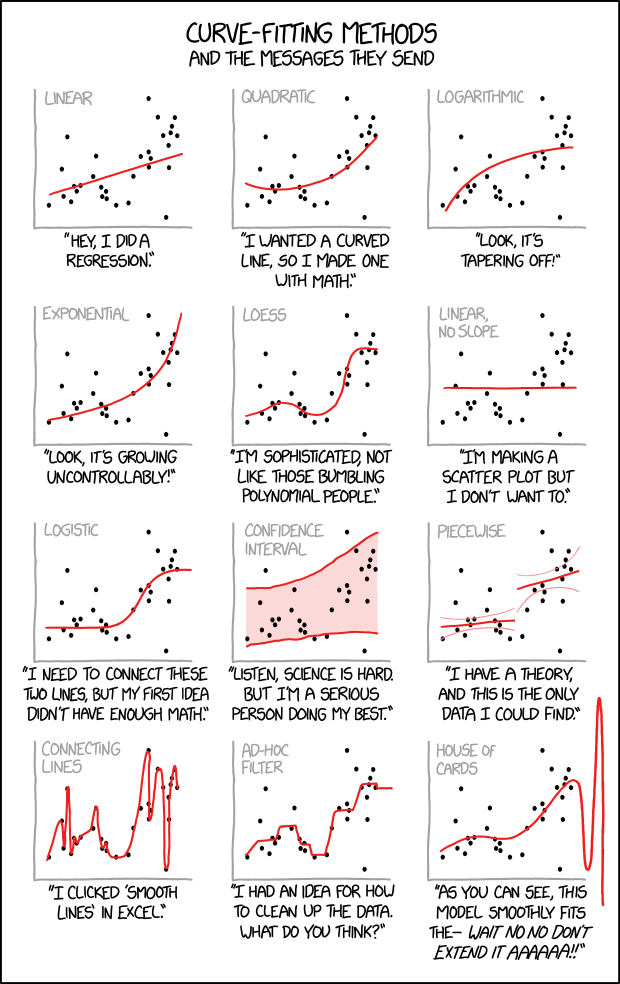
\includegraphics[width=\textwidth,height=0.65\textheight,keepaspectratio]{images/2048_curve_fitting.png}
\end{center}

\column{0.42\textwidth}
\vspace{8mm}
\small
\begin{compactlist}
\item Your dataset has 50 columns
\item You can only plot 2 axes
\item What do you do?
\end{compactlist}

\vspace{3mm}
\begin{block}{Today's Question}
\scriptsize How do we compress many features into a few while keeping the important patterns?
\end{block}
\end{columns}

\bottomnote{XKCD \#2048 by Randall Munroe (CC BY-NC 2.5). This is the problem we solve today.}
\end{frame}

%% ================================================================
%% ACT 1: "Your Data Has Too Many Dimensions"
%% ================================================================

%% ================================================================
%% SLIDE 3: 50 Features Scenario
%% ================================================================
\begin{frame}[t]{What Happens When You Have 50 Features?}
\small
A bank tracks \highlight{50 risk metrics} for each portfolio. A data scientist needs to visualize risk clusters.

\vspace{2mm}
\begin{compactlist}
\item Plotting 50 axes is impossible -- humans see at most 3 dimensions
\item Dropping features loses information -- which ones are safe to remove?
\item Many features are correlated -- they carry redundant information
\end{compactlist}

\vspace{2mm}
\begin{exampleblock}{The Key Insight}
\small What if there were \highlight{directions} in the data that capture most of the variation? Then we could project onto just those directions and lose almost nothing.
\end{exampleblock}

\vspace{2mm}
\scriptsize
This is exactly what \textbf{Principal Component Analysis (PCA)} does: it finds the directions of maximum variance and projects your data onto them.

\bottomnote{High-dimensional data is everywhere: genomics (20k genes), NLP (50k words), finance (hundreds of factors).}
\end{frame}

%% ================================================================
%% SLIDE 4: [CHART FIRST] High-D Before/After
%% ================================================================
\begin{frame}[t]{What Does Compressed Data Look Like?}
\begin{center}

\includegraphics[width=0.65\textwidth]{08_high_dim_before_after/chart.pdf}
\end{center}

\vspace{-2mm}
\small
\begin{compactlist}
\item Each dot was originally described by \highlight{10 numbers} (features)
\item PCA compressed it to just \highlight{2 numbers} (principal components)
\item The three clusters are still clearly visible after compression
\end{compactlist}

\bottomnote{PCA found the 2 directions that preserve the most spread in the data -- no human picked them.}
\end{frame}

%% ================================================================
%% SLIDE 5: Why Not Just Pick Two Features?
%% ================================================================
\begin{frame}[t]{Why Not Just Pick Two Features?}
\begin{columns}[T]
\column{0.47\textwidth}
\small
\textbf{\textcolor{mlred}{Cherry-Picking Features}}
\begin{compactlist}
\item Pick features 1 and 2 arbitrarily
\item Lose all information from features 3--10
\item The ``best'' pair depends on your task
\item You must try all $\binom{p}{2}$ pairs
\end{compactlist}

\column{0.47\textwidth}
\small
\textbf{\textcolor{mlgreen}{PCA Approach}}
\begin{compactlist}
\item Combine ALL features into 2 new axes
\item Each new axis is a weighted blend of all originals
\item Maximizes retained information automatically
\item No manual selection needed
\end{compactlist}
\end{columns}

\vspace{3mm}
\begin{block}{Key Difference}
\small PCA does not discard features -- it \highlight{blends} them. Each principal component is a linear combination of all original features.
\end{block}

\bottomnote{Selecting features = supervised (you choose). PCA = unsupervised (the data chooses).}
\end{frame}

%% ================================================================
%% SLIDE 6: What Does Variance Mean?
%% ================================================================
\begin{frame}[t]{What Does ``Variance'' Mean Here?}
\begin{columns}[T]
\column{0.50\textwidth}
\small
\textbf{The Formula}

\vspace{2mm}
$$\text{Var}(x) = \frac{1}{n}\sum_{i=1}^{n}(x_i - \bar{x})^2$$

\vspace{2mm}
\begin{compactlist}
\item Variance measures \highlight{spread} in the data
\item High variance = lots of information
\item Low variance = mostly noise
\end{compactlist}

\column{0.45\textwidth}
\vspace{2mm}
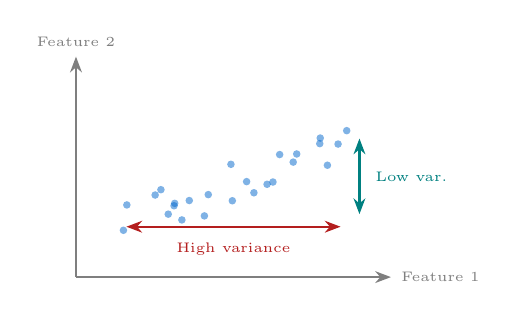
\begin{tikzpicture}[scale=0.8]
% Cloud of points with wide spread along one axis
\draw[-{Stealth[length=2mm]}, thick, mlgray] (0,0) -- (5,0) node[right, font=\tiny] {Feature 1};
\draw[-{Stealth[length=2mm]}, thick, mlgray] (0,0) -- (0,3.5) node[above, font=\tiny] {Feature 2};
% Elongated cloud
\foreach \i in {1,...,25} {
  \pgfmathsetmacro{\rx}{2.5 + 1.8*rand}
  \pgfmathsetmacro{\ry}{1.5 + 0.4*rand + 0.3*(\rx-2.5)}
  \fill[mlblue, opacity=0.5] (\rx, \ry) circle (0.06);
}
% Arrows showing variance
\draw[{Stealth[length=2mm]}-{Stealth[length=2mm]}, dfred, thick] (0.8,0.8) -- (4.2,0.8);
\node[font=\tiny, dfred, below] at (2.5,0.7) {High variance};
\draw[{Stealth[length=2mm]}-{Stealth[length=2mm]}, dfteal, thick] (4.5,1.0) -- (4.5,2.2);
\node[font=\tiny, dfteal, right] at (4.6,1.6) {Low var.};
\end{tikzpicture}
\end{columns}

\vspace{2mm}
\begin{alertblock}{}
\scriptsize In PCA, ``variance'' and ``information'' are treated as synonyms. This is an assumption, not a universal fact.
\end{alertblock}

\bottomnote{In PCA, ``variance'' and ``information'' are treated as synonyms. This is an assumption, not a fact.}
\end{frame}

%% ================================================================
%% SLIDE 7: Road Map
%% ================================================================
\begin{frame}[t]{Road Map: Three Steps of PCA}
\begin{columns}[T]
\column{0.50\textwidth}
\small
\begin{enumerate}
\setlength{\itemsep}{8pt}
\item \highlight{Center} the data\\
{\scriptsize Subtract the column mean from every feature so the cloud sits at the origin.}

\item \highlight{Find the directions} of maximum variance\\
{\scriptsize Compute the covariance matrix and its eigenvectors -- these are the principal components.}

\item \highlight{Project} onto those directions\\
{\scriptsize Multiply your data by the top $k$ eigenvectors to get $k$ new features.}
\end{enumerate}

\column{0.45\textwidth}
\vspace{4mm}
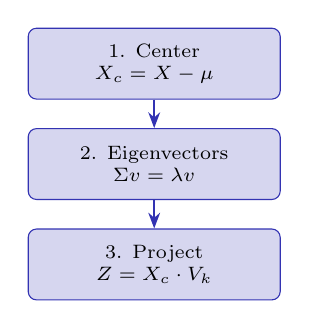
\begin{tikzpicture}[scale=0.85,
  box/.style={draw=mlpurple, fill=mllavender4, rounded corners=3pt, minimum width=3.2cm, minimum height=0.9cm, font=\scriptsize, align=center}]
\node[box] (s1) at (0,3) {1. Center\\$X_c = X - \mu$};
\node[box] (s2) at (0,1.5) {2. Eigenvectors\\$\Sigma v = \lambda v$};
\node[box] (s3) at (0,0) {3. Project\\$Z = X_c \cdot V_k$};
\draw[-{Stealth[length=2mm]}, mlpurple, thick] (s1) -- (s2);
\draw[-{Stealth[length=2mm]}, mlpurple, thick] (s2) -- (s3);
\end{tikzpicture}
\end{columns}

\vspace{3mm}
\begin{block}{}
\small That is the \highlight{entire algorithm}. We will see each step visually before any formulas.
\end{block}

\bottomnote{We will see each step visually before we see any formulas.}
\end{frame}

%% ================================================================
%% ACT 2: "PCA Finds the Directions That Matter"
%% ================================================================

%% ================================================================
%% SLIDE 8: [CHART FIRST] Principal Components
%% ================================================================
\begin{frame}[t]{Which Direction Captures the Most Spread?}
\begin{center}

\includegraphics[width=0.55\textwidth]{02_principal_components/chart.pdf}
\end{center}

\vspace{-2mm}
\small
\begin{compactlist}
\item The \highlight{first arrow (PC1)} points along the main cloud -- maximum spread
\item The \highlight{second arrow (PC2)} is perpendicular -- remaining spread
\item Together they form new coordinate axes for the data
\end{compactlist}

\bottomnote{PCA is a rotation: it does not distort your data, it views it from a better angle.}
\end{frame}

%% ================================================================
%% SLIDE 9: Step 1 - Center the Data
%% ================================================================
\begin{frame}[t]{Step 1: Center the Data}
\begin{columns}[T]
\column{0.48\textwidth}
\small
\textbf{Definition}

\vspace{2mm}
$$X_c = X - \mu$$

where $\mu = \frac{1}{n}\sum_{i=1}^{n} x_i$ is the column mean vector.

\vspace{3mm}
\begin{compactlist}
\item Subtract the mean of each feature
\item The centered cloud sits at the origin
\item Ensures PC1 passes through the center of the data
\end{compactlist}

\column{0.48\textwidth}
\small
\textbf{Mini-Example}

\vspace{2mm}
\scriptsize
Data: $(2,4),\;(4,6),\;(6,8),\;(8,10)$

Mean: $\mu = (5, 7)$

\vspace{1mm}
Centered:
\begin{tabular}{@{}cc@{}}
\toprule
$x_1 - 5$ & $x_2 - 7$ \\
\midrule
$-3$ & $-3$ \\
$-1$ & $-1$ \\
$+1$ & $+1$ \\
$+3$ & $+3$ \\
\bottomrule
\end{tabular}

\vspace{2mm}
\small The cloud shifts so its center is at $(0,0)$.
\end{columns}

\bottomnote{Centering ensures PC1 passes through the origin. Without centering, the mean dominates the first component.}
\end{frame}

%% ================================================================
%% SLIDE 10: Step 2 - Covariance Matrix
%% ================================================================
\begin{frame}[t]{Step 2: The Covariance Matrix}
\begin{columns}[T]
\column{0.48\textwidth}
\small
\textbf{Formula}

\vspace{2mm}
$$\Sigma = \frac{1}{n-1} X_c^T X_c$$

\vspace{2mm}
This is a $p \times p$ matrix where $p$ is the number of features.

\vspace{2mm}
\begin{compactlist}
\item Diagonal entries = variance of each feature
\item Off-diagonal entries = how features move together
\end{compactlist}

\column{0.48\textwidth}
\small
\textbf{Interpretation}

\vspace{2mm}
$$\Sigma = \begin{pmatrix} \text{Var}(x_1) & \text{Cov}(x_1,x_2) \\ \text{Cov}(x_2,x_1) & \text{Var}(x_2) \end{pmatrix}$$

\vspace{3mm}
\begin{compactlist}
\item Large off-diagonal = features are redundant
\item Redundancy = PCA can compress
\item All zeros off-diagonal = features already independent, PCA does nothing
\end{compactlist}
\end{columns}

\bottomnote{If all off-diagonals were zero, PCA would do nothing -- the features are already independent.}
\end{frame}

%% ================================================================
%% SLIDE 11: Step 3 - Eigenvalues and Eigenvectors
%% ================================================================
\begin{frame}[t]{Step 3: Eigenvalues and Eigenvectors (The Key Equation)}
\begin{columns}[T]
\column{0.48\textwidth}
\small
\textbf{The Equation}

\vspace{2mm}
$$\Sigma \, v = \lambda \, v$$

\vspace{2mm}
\begin{compactlist}
\item $v$ is an \highlight{eigenvector}: a direction that $\Sigma$ only stretches, never rotates
\item $\lambda$ is the \highlight{eigenvalue}: how much it stretches (= variance along $v$)
\item Largest $\lambda$ = most important direction
\end{compactlist}

\column{0.48\textwidth}
\small
\textbf{Intuition}

\vspace{2mm}
Imagine pulling a rubber sheet anchored at the center:

\vspace{2mm}
\begin{compactlist}
\item The eigenvectors are the directions that \highlight{only stretch}, not twist
\item The eigenvalues tell you \highlight{how far} each direction stretches
\item We keep the directions that stretch the most
\end{compactlist}

\vspace{2mm}
\begin{block}{}
\scriptsize This is the ONLY equation you need to remember. Everything else follows from it.
\end{block}
\end{columns}

\bottomnote{This is the ONLY equation you need to remember. Everything else follows from it.}
\end{frame}

%% ================================================================
%% SLIDE 12: Derivation
%% ================================================================
\begin{frame}[t]{Derivation: Why Does PCA Maximize Variance?}
\small
We want the direction $v$ that maximizes the variance of the projected data:

\vspace{2mm}
\begin{enumerate}
\setlength{\itemsep}{4pt}
\item \textbf{Objective:} Maximize $\text{Var}(X_c \, v) = v^T \Sigma \, v$
\item \textbf{Constraint:} $\|v\| = 1$ \;\;(unit length, so the answer is a direction, not a scale)
\item \textbf{Lagrangian:} $\mathcal{L} = v^T \Sigma \, v - \lambda(v^T v - 1)$
\item \textbf{Set derivative to zero:} $\frac{\partial \mathcal{L}}{\partial v} = 2\Sigma v - 2\lambda v = 0 \;\;\Rightarrow\;\; \Sigma v = \lambda v$
\end{enumerate}

\vspace{3mm}
\begin{block}{Result}
\small The eigenvectors of $\Sigma$ are the principal components. The eigenvalues are their variances. The \highlight{largest eigenvalue} corresponds to the direction of maximum variance (PC1).
\end{block}

\bottomnote{Pearson (1901) and Hotelling (1933). The constrained optimization is standard Lagrange multipliers.}
\end{frame}

%% ================================================================
%% SLIDE 13: Worked Example
%% ================================================================
\begin{frame}[t]{Worked Example: 2D to 1D by Hand}
\small
\textbf{Data:} 5 points in 2D: $(1,2),\;(3,4),\;(5,6),\;(2,3),\;(4,5)$

\vspace{1mm}
\textbf{Step 1 -- Center:} $\mu = (3, 4)$. Centered: $(-2,-2),\;(0,0),\;(2,2),\;(-1,-1),\;(1,1)$

\vspace{1mm}
\textbf{Step 2 -- Covariance:}
$\Sigma = \frac{1}{4}\begin{pmatrix} 10 & 10 \\ 10 & 10 \end{pmatrix} = \begin{pmatrix} 2.5 & 2.5 \\ 2.5 & 2.5 \end{pmatrix}$

\vspace{1mm}
\textbf{Step 3 -- Eigenvalues:} $\det(\Sigma - \lambda I) = 0 \;\Rightarrow\; \lambda_1 = 5,\;\lambda_2 = 0$

\vspace{1mm}
\textbf{Eigenvector for $\lambda_1 = 5$:} $v_1 = \frac{1}{\sqrt{2}}(1, 1)$ \;(the 45-degree line)

\vspace{1mm}
\textbf{Project:} $z_i = v_1^T x_{c,i}$: $\;-2\sqrt{2},\;0,\;2\sqrt{2},\;-\sqrt{2},\;\sqrt{2}$

\vspace{2mm}
\begin{block}{Result}
\small We reduced 2D to 1D and kept \highlight{100\%} of the variance ($\lambda_2 = 0$ means the second direction had zero spread -- the data was perfectly correlated).
\end{block}

\bottomnote{Try this yourself: change the correlation and watch how the PC direction rotates.}
\end{frame}

%% ================================================================
%% SLIDE 14: [CHART FIRST] Biplot
%% ================================================================
\begin{frame}[t]{How Do You Read a Biplot?}
\begin{center}

\includegraphics[width=0.60\textwidth]{top10_10_pca_biplot/chart.pdf}
\end{center}

\vspace{-2mm}
\small
\begin{compactlist}
\item \highlight{Dots} = data points in PC space
\item \highlight{Arrows} = original features. Long arrow = feature contributes strongly
\item Arrows pointing the same direction = correlated features
\end{compactlist}

\bottomnote{Biplots are the main diagnostic tool for interpreting what PCA did. Always plot one.}
\end{frame}

%% ================================================================
%% SLIDE 15: [CHART FIRST] Scaling Effect
%% ================================================================
\begin{frame}[t]{What Happens If You Forget to Scale?}
\begin{center}

\includegraphics[width=0.55\textwidth]{top10_11_scaling_effect/chart.pdf}
\end{center}

\vspace{-2mm}
\small
\begin{compactlist}
\item \highlight{Without scaling}: a feature measured in thousands dominates PC1 alone
\item \highlight{After scaling}: all features contribute fairly to each component
\item Always standardize unless features share the same units
\end{compactlist}

\bottomnote{StandardScaler (zero mean, unit variance) is the default. Skip it only when features are already on the same scale.}
\end{frame}

%% ================================================================
%% SLIDE 16: [CHART FIRST] Cluster Separation
%% ================================================================
\begin{frame}[t]{Can PCA Separate Clusters?}
\begin{center}

\includegraphics[width=0.60\textwidth]{06b_pca_cluster_projection/chart.pdf}
\end{center}

\vspace{-2mm}
\small
\begin{compactlist}
\item Each color is a different class. PCA separates some but not all
\item Well-separated classes remain distinct; overlapping classes stay mixed
\item PCA is \highlight{linear} -- it cannot untangle nonlinear structure
\end{compactlist}

\bottomnote{For better cluster separation on complex data, consider t-SNE (visualization) or UMAP.}
\end{frame}

%% ================================================================
%% SLIDE 17: When Does PCA Fail?
%% ================================================================
\begin{frame}[t]{When Does PCA Fail?}
\begin{columns}[T]
\column{0.47\textwidth}
\small
\textbf{\textcolor{mlgreen}{Strengths}}
\begin{compactlist}
\item Linear relationships between features
\item Correlated features (high redundancy)
\item Preprocessing for ML pipelines
\item Interpretable components (loadings)
\end{compactlist}

\column{0.47\textwidth}
\small
\textbf{\textcolor{mlred}{Weaknesses}}
\begin{compactlist}
\item Nonlinear structure (e.g., swiss roll)
\item Sensitive to outliers (they inflate variance)
\item All features must be numeric
\item Components are blends, not single features
\end{compactlist}
\end{columns}

\vspace{4mm}
\begin{alertblock}{The Linear Assumption}
\small PCA assumes linear relationships. If your data lives on a curved surface, PCA will cut through it rather than follow the curve.
\end{alertblock}

\bottomnote{PCA assumes linear relationships. If your data lives on a curved surface, PCA will cut through it.}
\end{frame}

%% ================================================================
%% SLIDE 18: PCA as Preprocessing
%% ================================================================
\begin{frame}[t]{PCA as Preprocessing: The 95\% Rule}
\small
\textbf{Practical Recipe for Using PCA in a Machine Learning Pipeline}

\vspace{3mm}
\begin{enumerate}
\setlength{\itemsep}{4pt}
\item \textbf{Scale:} \texttt{StandardScaler().fit\_transform(X)}
\item \textbf{Reduce:} \texttt{PCA(n\_components=0.95).fit\_transform(X\_scaled)}
\item \textbf{Model:} Feed the reduced data into your classifier or regressor
\end{enumerate}

\vspace{3mm}
\begin{block}{How It Works}
\small When you pass \texttt{n\_components=0.95}, sklearn \highlight{automatically selects $k$} -- the smallest number of components that explain at least 95\% of total variance. No manual scree plot needed.
\end{block}

\vspace{2mm}
\scriptsize
\textbf{Why does this help?} PCA removes noise dimensions, so downstream models train faster and often achieve \emph{better} accuracy (less overfitting from irrelevant features).

\bottomnote{PCA before KNN or logistic regression often improves speed AND accuracy by removing noise dimensions.}
\end{frame}

%% ================================================================
%% ACT 3: "How Well Did It Work?"
%% ================================================================

%% ================================================================
%% SLIDE 19: [CHART FIRST] Scree Plot
%% ================================================================
\begin{frame}[t]{How Many Components Do We Keep?}
\begin{center}

\includegraphics[width=0.60\textwidth]{01_scree_plot/chart.pdf}
\end{center}

\vspace{-2mm}
\small
\begin{compactlist}
\item \highlight{Bars} = variance explained by each PC. The first few tower over the rest
\item \highlight{Line} = cumulative variance. It crosses 80\% quickly
\item The \highlight{elbow} says: keep components before the curve flattens, discard the rest
\end{compactlist}

\bottomnote{Named after geological ``scree'' (rubble at a cliff base). You stop where the cliff flattens into rubble.}
\end{frame}

%% ================================================================
%% SLIDE 20: Rules of Thumb for Choosing k
%% ================================================================
\begin{frame}[t]{Rules of Thumb for Choosing $k$}
\begin{columns}[T]
\column{0.30\textwidth}
\small
\textbf{1. Elbow Method}
\begin{compactlist}
\item Look at the scree plot
\item Find where the curve ``bends''
\item Keep components before the elbow
\end{compactlist}

\column{0.30\textwidth}
\small
\textbf{2. Threshold Method}
\begin{compactlist}
\item Set a target: 90--95\% variance
\item Count components needed to reach it
\item Simple and widely used
\end{compactlist}

\column{0.30\textwidth}
\small
\textbf{3. Cross-Validation}
\begin{compactlist}
\item Pick $k$ that maximizes downstream task performance
\item Most principled approach
\item Requires a supervised task
\end{compactlist}
\end{columns}

\vspace{4mm}
\begin{block}{}
\small No single rule is always best. In practice, try 2--3 methods and see if they agree.
\end{block}

\bottomnote{No single rule is always best. In practice, try 2--3 methods and see if they agree.}
\end{frame}

%% ================================================================
%% SLIDE 21: [CHART FIRST] Reconstruction Error
%% ================================================================
\begin{frame}[t]{Reconstruction Error: What Did We Lose?}
\begin{center}

\includegraphics[width=0.60\textwidth]{03_reconstruction/chart.pdf}
\end{center}

\vspace{-2mm}
\small
\begin{compactlist}
\item Error drops steeply for the first few components
\item After $k \approx 5$, adding components barely helps
\item The gap between $k{=}3$ and $k{=}20$ is only a few percent
\end{compactlist}

\bottomnote{Reconstruction: $\hat{X} = Z \cdot V_k^T + \mu$. The error is $\|X - \hat{X}\|^2$.}
\end{frame}

%% ================================================================
%% SLIDE 22: [CHART FIRST] Yield Curve PCA
%% ================================================================
\begin{frame}[t]{Finance Application: Yield Curve PCA}
\begin{center}

\includegraphics[width=0.60\textwidth]{09_yield_curve_factors/chart.pdf}
\end{center}

\vspace{-2mm}
\small
\begin{compactlist}
\item \highlight{PC1} (flat bars) = all maturities move together = ``Level''
\item \highlight{PC2} (sloped bars) = short and long rates diverge = ``Slope''
\item \highlight{PC3} (U-shaped bars) = belly moves differently = ``Curvature''
\end{compactlist}

\bottomnote{Litterman \& Scheinkman (1991): 3 PCA factors explain $>$98\% of US Treasury yield curve movements.}
\end{frame}

%% ================================================================
%% SLIDE 23: Yield Curve Worked Numbers
%% ================================================================
\begin{frame}[t]{Yield Curve PCA: The Worked Numbers}
\begin{columns}[T]
\column{0.48\textwidth}
\small
\textbf{Portfolio Risk with PCA}

\vspace{2mm}
Instead of tracking 5+ maturity exposures, use 3 factor sensitivities:

\vspace{2mm}
$$\Delta P \approx D_1 \cdot \Delta\text{PC1} + D_2 \cdot \Delta\text{PC2} + D_3 \cdot \Delta\text{PC3}$$

\vspace{2mm}
where $D_k$ = sensitivity (``factor duration'') to factor $k$.

\column{0.48\textwidth}
\small
\textbf{Example}

\vspace{2mm}
\scriptsize
Suppose:
\begin{compactlist}
\item Level shifts $+10$bp (PC1 $= +10$)
\item Slope steepens (PC2 $= +5$)
\item Curvature unchanged (PC3 $= 0$)
\item $D_1 = 0.8,\; D_2 = 0.3,\; D_3 = 0.1$
\end{compactlist}

\vspace{2mm}
\small
Then:

$\Delta P \approx 0.8 \times 10 + 0.3 \times 5 + 0.1 \times 0$

$\phantom{\Delta P} = 8.0 + 1.5 + 0 = \highlight{9.5\text{bp}}$
\end{columns}

\vspace{2mm}
\begin{block}{}
\small 3 numbers replace 5+ maturity exposures. This is why every fixed income desk uses PCA.
\end{block}

\bottomnote{3 numbers replace 5+ maturity exposures. This is why every fixed income desk uses PCA.}
\end{frame}

%% ================================================================
%% SLIDE 24: PCA Decision Checklist
%% ================================================================
\begin{frame}[t]{PCA Decision Checklist}
\begin{columns}[T]
\column{0.47\textwidth}
\small
\textbf{\textcolor{mlgreen}{Use PCA When\ldots}}
\begin{compactlist}
\item Features are correlated (large off-diagonals in $\Sigma$)
\item Too many dimensions for your model or plot
\item Preprocessing to speed up ML and reduce noise
\item You want interpretable compression (loadings)
\end{compactlist}

\column{0.47\textwidth}
\small
\textbf{\textcolor{mlred}{Skip PCA When\ldots}}
\begin{compactlist}
\item Few features already ($p < 10$)
\item Nonlinear structure (use kernel PCA or t-SNE)
\item You need original feature names in the output
\item Data is categorical (PCA needs numeric inputs)
\end{compactlist}
\end{columns}

\vspace{4mm}
\begin{block}{Quick Test}
\small The simplest test: if your \highlight{correlation matrix has large off-diagonal entries}, PCA will help. If features are already independent, PCA adds nothing.
\end{block}

\bottomnote{The simplest test: if your correlation matrix has large off-diagonal entries, PCA will help.}
\end{frame}

%% ================================================================
%% SLIDE 25: Closing Summary + XKCD
%% ================================================================
\begin{frame}[t]{PCA in Four Sentences}
\begin{columns}[T]
\column{0.53\textwidth}
\small
\vspace{2mm}
\begin{enumerate}
\setlength{\itemsep}{6pt}
\item High-dimensional data is hard to visualize and model
\item PCA finds orthogonal directions of maximum variance
\item Keep $k$ components that explain 90--95\% of variance
\item In finance, 3 PCA factors explain nearly all yield curve movement
\end{enumerate}

\vspace{3mm}
\begin{block}{Next Steps}
\scriptsize Explore t-SNE for nonlinear visualization in the deep dive. Try the Jupyter notebook to run PCA on real financial data.
\end{block}

\column{0.42\textwidth}
\vspace{2mm}
\begin{center}
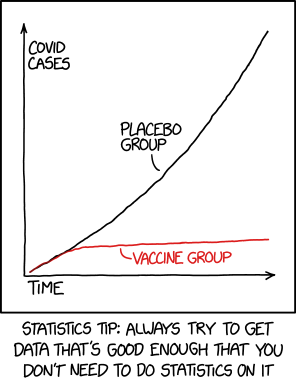
\includegraphics[width=\textwidth,height=0.60\textheight,keepaspectratio]{images/2400_statistics.png}
\end{center}
\end{columns}

\bottomnote{XKCD \#2400 by Randall Munroe (CC BY-NC 2.5). Next: explore t-SNE for nonlinear visualization in the deep dive.}
\end{frame}

\end{document}
